\vspace{10pt}

{\centering\subsection*{刘笑:小猫}}

\addcontentsline{toc}{subsection}{刘笑:小猫}

\renewcommand{\leftmark}{刘笑:小猫}

\begin{figure}[htbp]

\centering

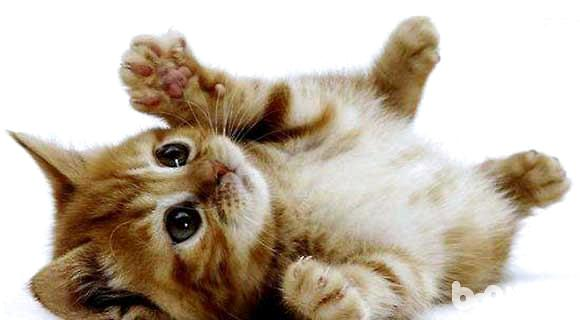
\includegraphics[width = .5\textwidth]{./ch/28.jpg}

\end{figure}




你们的动物朋友是什么呢?我的动物朋友有很多很多,但其中我最喜欢的是只小猫。



这只猫的毛是半黄半白的,它左眼有一圈黄色的毛,右脚那有一块黑色的斑,显得它更加可爱了。它跟别的猫可不一样,别的猫爱吃鱼,可这只猫只吃蔬菜面条,它可真是一只特别的猫啊!更让人着迷的还是它那一双水汪汪的眼睛,仿佛是一颗颗闪闪亮亮的宝石。



这只小猫仿佛通灵性。它会在你无聊的时候陪你玩耍,在你不开心时逗你开心,每当你放学回家它便会在家门口等你。



它要是高兴就会用身子蹭你的腿,让你给它抓痒,还会会逗你玩。它要是不高兴,无论谁说多少好话,它也总是板着张脸,对你爱搭不搭。



它还是抓老鼠的专家,它要是听见老鼠发出一点声音,它就立刻警戒起来,躲在桌椅后面等待时机。



这就是我的动物朋友,你们喜欢我的动物朋友吗?





\vspace{10pt}



作者:四(2)班 刘笑



指导老师:陈小丽



投稿:2021年4月27日



发表:2021年5月10日








                



\vspace{10pt}

\hline



